\documentclass{article} 
\usepackage{graphicx,subcaption} %allows for includuing figures in LaTeX document
\graphicspath{{/Users/E31345/Desktop/LaTeX_figs/}} %Setting the graphicspath
\usepackage{float}
\usepackage[compact]{titlesec}  
\titlespacing{\section}{2pt}{2pt}{2pt}
\usepackage[export]{adjustbox}
% adjust margins
\usepackage[margin=1.25in]{geometry}
%add dot to section numbers
\usepackage{titlesec}
\titlelabel{\thetitle.\quad}
% numbering paragraphs code
\newcounter{para}
\newcommand\mypara{\par\refstepcounter{para}\textbf{[\thepara]}\space}
%Preamble 
% need to provide annotations with organizational affiliations for authors
\author{R. J. Irvin, R. H. Varney, A. S. Reimer, P. M. Reyes, and S. R. Kaeppler}
% need left justified
\title{A Statistical Study of Energetic Particle Precipitation in the D-Region Ionosphere using PFISR}
\date{May 2018}

%content
\begin{document}

\maketitle


\mypara Energetic particles trapped in the inner magnetosphere can, as a result of wave-particle interactions, enter the loss cone and precipitate into the atmosphere. Only the most energetic of these particles can reach penetration depths in the D-region, causing enhanced ionization that can be detected by ISR's. These particles and the enhanced ionization they cause can damage satellites and disrupt radio transmissions. 
*[Something about needing to do longterm study, difficulty of in situ measurements, etc.]*
Using PFISR D-region data from 2009-2018 we developed a method to identify events of enhanced ionization caused by energetic particle precipitation, and observed how the frequency of these events scale with geomagnetic activity, MLT, and F-region convection currents measured by PFISR.
We found that energetic particle precipitation is more likely on the dawn side, the period of 0-12 MLT, for higher global AE values and during substorms. We also note higher likelihood of energetic particle precipitation near 18 MLT during the late recovery phase of substorms and a strong bias for eastward convection currents which agrees with our 0-12 MLT result.
Comparing our results with global distribution studies of some plasmaspheric waves suggests that whistler mode chorus waves contribute to energetic particle precipitation into the D-region during periods of high geomagnetic activity. 
%Intro
\section{Introduction}
\mypara Parameterizations of electron impact ionization suggest that incident energetic electron precipitation with energies $\geq$ 30 keV will result in regions of enhanced electron density in the D-region Ionosphere [Fang:2008,Fang:2010]
*[What belongs in the introduction for this paper? Maybe a lot of the stuff I include in the Methodology like PFISR experiment params?]*




\section{Instrumentation}
\mypara All of our data for this study was acquired from PFISR D-region modes so it is worth discussing them at length. *[defer/cite to the niccols 2010 for a lot of this]*. Include discussion of D-region modes and their experimental parameters, L shell, magnetic latitude, define Nyquist frequency (from IPP), beam look directions, barker code, Noise estimation, Power transmitted, and what is received. This will segway into Thomson scattering of single electrons into kudeki. Present the electron spectral density in collisional regime derived by kudeki (lorentzian) and discuss ion diffusion coefficient scaling with neutral density and neutral density increases exponentially with decreasing altitude  so spectral width decreases with altitude *[Roger mentioned I could actually model the expected ESD (electron spectral density) with altitude from the coefficients given in Schunk and compare to what we actually see. Temperature dependent but shouldn't affect that much]*. Present ACF/spectra plot, we may omit the ACF in which case present the Lorentzian looking spectra side by side. Explain the significance of 85 km, this is the altitude where the spectral width of the ESD is about the nyquist frequency, so spectra basically look flat above this (why, show modeled from Schunk coefficients?)
\section{Methodology}
\mypara Before describing the method developed to identify events of enhanced electron density resulting from energetic particle precipitation, we must first introduce the PFISR D-region mode used for these experiments as well as the expected ISR electron density spectra in the collisional regime. *[ Provide relevant PFISR and MSwinds23 specs (L=5.7,2ms IPP,13 baud barker code, beam directions/resolution, Power transmitted, nyquist, etc.)]*. This particular D-region mode has been run without taking dedicated noise samples, as a result we had to estimate the time-dependent noise in each beam by averaging the spectra over 'dark' altitudes. That is, altitudes which are below any expected enhanced ionization, but above the ground clutter picked up by PFISR. *[Do i need to define/describe ground clutter in general or for PFISR in particular?]*. Thus, we use the altitude range 52.5-57.5 km for our noise samples. Note: this is not exactly precise, as range aliasing from the upper F-region and malfunctioning antennas in the phased array caused the noise in this range to be slightly overestimated and this is clear when experiments in which PFISR did not detect any electron density enhancements were analyzed. However, this overestimation in the noise is negligible for experiments with these enhancements *[Do I provide a figure or simple calculation to prove this, i.e. deviation in the noise / average real signal?, or is this too much discussion on the matter?]*.
\mypara Neutral densities in the D-region are far greater than that in the E or F regions *[citation]* and therefor  interactions are dominated by collisions*[explain what it means to be dominated by collisions, i.e. more likely to recombine with positive ions]*. In the collisional regime the expected ISR power spectrum is a lorenztian [Kudeki:2011]. Equation [\ref{eqn:kudeki}] can be found in [Kudeki:2011] as equation 50
\begin{equation}
	\frac{\left<\left|n_e\left(\textbf{k},\omega\right)\right|^2\right>}{N_o}  \approx \frac{2k^2D_i}{(\omega-\omega_o)^2+\left(2k^2D_i\right)^2} 
	\label{eqn:kudeki}
\end{equation}
Where the LHS is the electron density power spectrum and $D_i=\frac{KT_i}{m_i\nu_i}$ is the ion diffusion coefficient in the collisional plasma. Thus we see that the electron density spectrum should narrow with decreasing altitude as the ion collision rate increases *[citation. How does ion collision rate increase?]*. 
We begin with the electron spectral densities for each time, beam, and altitude *[discuss how we get these spectra, the fitter, processing code, etc.?]*. From discussion on the ISR spectrum in the highly collisional regime, events with EED (enhanced electron density) in the D-region due to EPP (energetic particle precipitation) should be marked by the spectral width of the electron density spectrum decreasing with altitude *[We should discuss this further, I don't think this is really a sufficient explanation. Misunderstanding Kudeki's derivation?]*. Equivalently, we can make sense of this result in time domain with the ACF's and looking at how the decorrelation times vary with altitude. The expected auto-correlation function of a Lorentzian in the frequency domain is an exponential decay function like $e^{-\frac{\left|\tau\right|}{\tau_c}}$ *[define terms/citation/derivation?*]. Figure [\ref{fig:acf}] shows these relations by plotting the uncalibrated electron spectral density, the normalized ACFs at 80 km with a fitted exponential decay curve, and the unnormalized ACFs across all D-region altitudes and beams for an experiment run on May 8 2017, which is one will look at throughout this paper *[define look directions of the beams here? do I need to discuss my reasons for picking this particular experiment or explain further what we are seeing here?]*.
%acf fig
\begin{figure}[t] % ! overrides latex, h here, t top, b bottom, p special page for floating objects
	\centering
	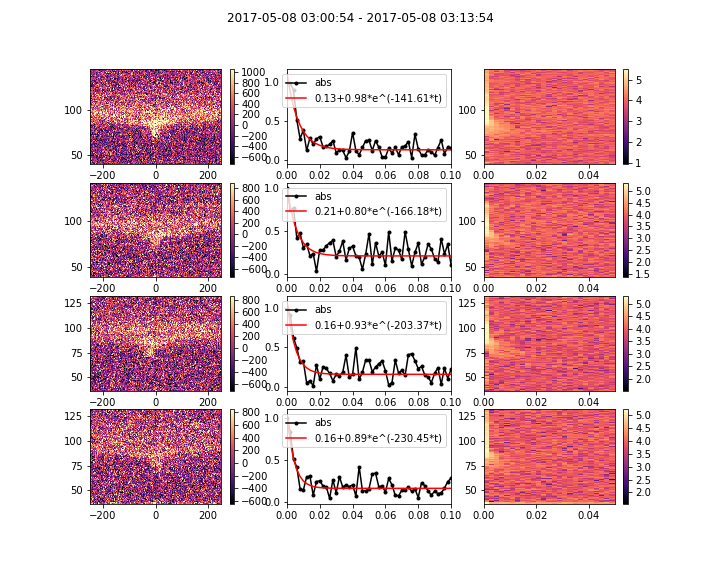
\includegraphics[scale=0.5]{ACF}
	 % adding right pushes my fig to the left wtf
	\caption[Short caption]{\textit{D-region experiment showing EED at 16 MLT. column i) shows 13 minute integrated uncalibrated electron spectral density. Column iii) shows unnormalized decorrelation times for each beam as a function of altitude. Column ii) shows the normalized ACF magnitude for each beam at 80 km with a fitted curve *define beam look directions here or earlier?*}}
	\label{fig:acf}
\end{figure}
%end acf fig
\mypara The best way to parameterize the spectral width of the measured electron spectral densities would be to apply a non-linear fitting algorithm; fitting a Lorentzian with variable noise floor (taking care of our lack of noise samples problem) and determining the spectral width of the fitted curve. However, this process is computationally expensive and we wanted a cheap method, good to first order, that could summarize the relevant details, as they pertain to EPP, of PFISR D-region experiments. Thus we use the first three moments of the measured electron spectral densities, which provide efficient calculations of the power, radial doppler shift, and the square of the spectral width given by equations \ref{eqn:power} through \ref{eqn:specwidth} *[citations/better explanations for the last three sentences*]. Note: in actual calculations these integrals are discrete sums from -256 to 256 Hz with resolution of *[explain these numbers]*. 
% in the next section define the three moment equations
\begin{equation}
	N_e=\int S(f)df
	\label{eqn:power}
\end{equation}
\begin{equation} %doppler eqn
	\bar{f}=\frac{\int fS(f)df}{N_e}
	\label{eqn:doppler}
\end{equation}
\begin{equation} %specwidth eqn
	\bigtriangleup f^2=\frac{\int (f-\bar{f})S(f)df}{N_e}
	\label{eqn:specwidth}
\end{equation}
% identify figure
\begin{figure}[h] % ! overrides latex, h here, t top, b bottom, p special page for floating objects	
	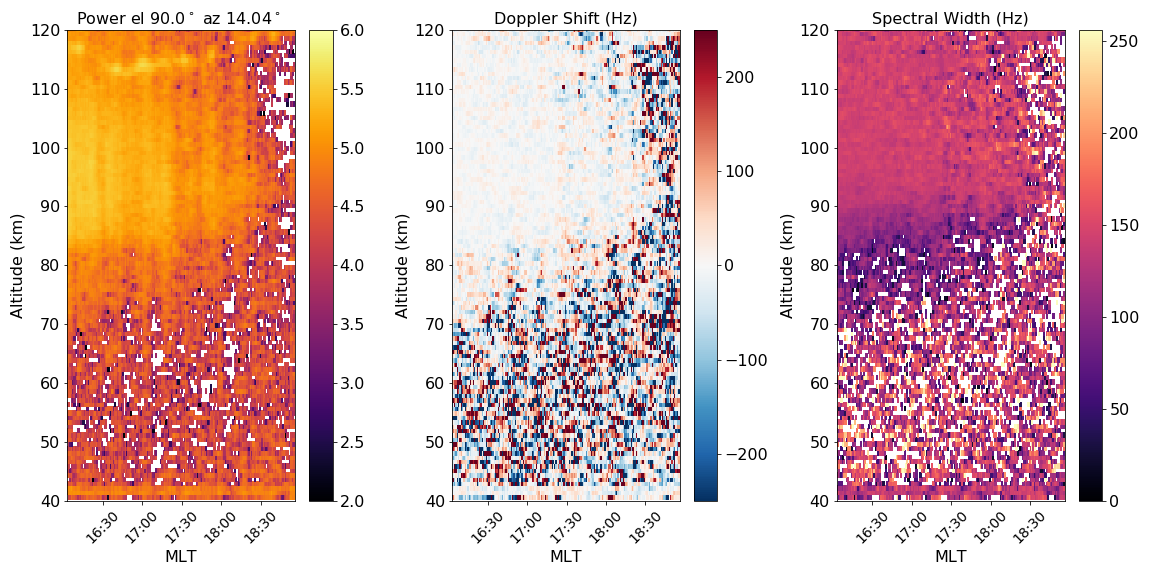
\includegraphics[width=\textwidth]{identify} % adding right pushes my fig to the left wtf
	\caption[Short caption]{\textit{Moment plots for up and up B look directions}}
	\label{fig:id}
\end{figure}
The 5 minute integrated power, doppler shift, and spectral width plots for the May 8, 2017 experiment are shown in Figure \ref{fig:id}. Measurements were taken between 1600-1900 MLT and plots are only displayed for two of the four beams, perpendicular to the ground and along the magnetic field line at PFISR. Notice in the spectral width plot, the decreasing of the spectral width with respect to altitude, particularly below 85 km during the first two hours of the experiment. This is what we are looking for, the narrowing of the electron spectral density, and classifying as EPP *[What is the significance of 85 km again?]*. This power plot is picking up a sporadic E layer, PMSE are also visible during some experiments, and the doppler plot can give a qualitative view of the radial wind velocities in an experiment *[How much do i discuss power and doppler, because spec width is the star of the show right?]*
% Describe by hand method
\mypara *[Now discuss the process of going through experiments, what I did/what i looked for, ones and zeros by hand in 30 minute bins, and discuss bias in experiments. Some other useful figures or data about the daily, yearly, monthly, hourly distribution of experiments? Include conjunctions with satellites or is that beyond the scope of this study?? Mention still missing some mswinds rand and some newer D-region experiments from 2018 which make my results better]*
\mypara *[Discuss/describe what geomag indices we looked at and why. F10.7-solar cycle, Dst - substorms, AE - aurora. Mention where I got my data (Kyoto citation). Discuss precipitation percentage calculation including precipitation timescale issue, i.e. we are using 5 min integration and 30 minute bins]*


\section{Results}
\mypara Though we recorded our observed EPP data in 30 minute intervals, here we present our plots with one hour resolution to increase the sample size, and therefor the confidence, in each bin. In Figure \ref{fig:ae:ae} the ranges of the first few bins are arbitrary, they were selected so as to flatten out the sampling distribution *[is this wrong, are there other interesting AE ranges]*except for the final bin, which contains events during high geomagnetic activity, AE $>$250 nT. Notable results are high levels of precipitation on the dawn side during periods of high geomagnetic activity, it is worth noting that not many events are available from 0500 to 1100 MLT. The regions of 30-50 nT and 50-100 nT have relative maxima in observed EPP during 1400-1600 MLT *[EMIC waves dusk side? late recovery phase of substorms?]*.  \mypara Observed EPP is comparatively uniform across MLT and F10.7 in \ref{fig:ae:f107} with the exception of near 0 observation percentage on the night side for small F10.7. It is worth noting that this period lines up with a minimum in observation events so deeper investigation into this population is require *[Explanation? Bias in events with low F10.7?]*. Interesting that 0000-0600 MLT for 75-90 bin has fairly high precipitation percentage.  Near noon is a local max all the way around. Transition to dusk seems to be steepest drop off in precipitation percentage. 
\mypara Now we turn our attention to Dst in Figure \ref{dst} Bins were selected with bit more care. 30 is upper limit and the 5 to 30 bin denotes significantly positive Dst values. -5 to 5 bin is the statistically 0 bin based on uncertainty in instrument measurements *[citation]*. -20 to -110 is significantly negative bin, note the Air Force's definition of substorm is below -75 *[citation, this only qualifies to 3 experiments]*.  Like with AE, there is more observed EPP on the dawn side for higher (more negative) Dst values.  There is also an interesting population around 1600-1800 MLT in region of -10 to -20 Dst. This is one to two hours after spike in AE 30-100 nT bin. Takes one hour for chorus waves to create pancake distributions by scattering electrons injected from plasma sheet into the loss cone [Thorne:2010]. *[Probably not related]*
% AE/F10.7 results figure
\begin{figure}
    \centering
    \begin{subfigure}[h]{0.48\linewidth}        %% or \columnwidth
        \centering
        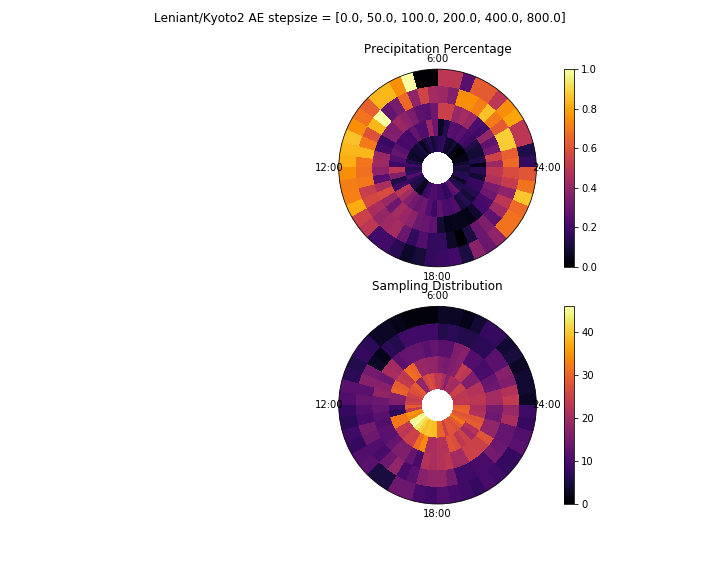
\includegraphics[width=\linewidth]{AEleniant-kyoto2}
        \caption{Caption A}
        \label{fig:ae:ae}
    \end{subfigure}
    \begin{subfigure}[h]{0.48\linewidth}        %% or \columnwidth
        \centering
        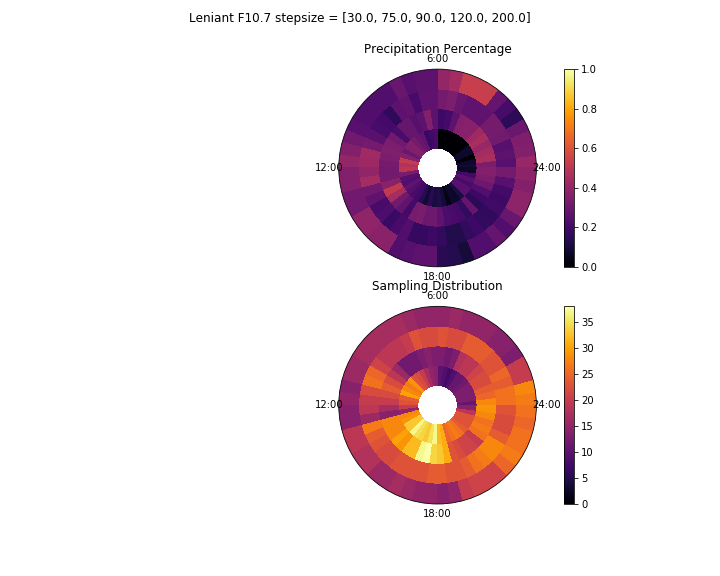
\includegraphics[width=\linewidth]{F107leniant}
        \caption{Caption B}
        \label{fig:ae:f107}
    \end{subfigure}
    \caption{AE/F10.7}
    \label{fig:ae}
\end{figure}
%DST results figure
\begin{figure}
    \centering
    \begin{subfigure}[h]{0.3\linewidth}        %% or \columnwidth
        \centering
        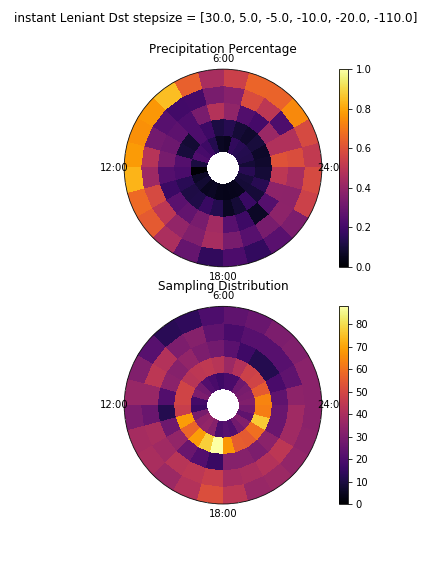
\includegraphics[width=\linewidth]{DSTinstant}
        \caption{Instantaneous Dst}
        \label{fig:dst:a}
    \end{subfigure}
    \begin{subfigure}[h]{0.3\linewidth}        %% or \columnwidth
        \centering
        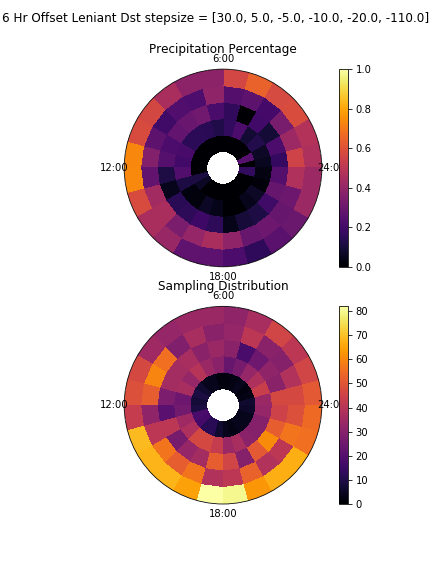
\includegraphics[width=\linewidth]{6DstOffsetStrict}
        \caption{Minimum Dst 6 hours prior}
        \label{fig:dst:b}
    \end{subfigure}
       \begin{subfigure}[h]{0.3\linewidth}        %% or \columnwidth
        \centering
        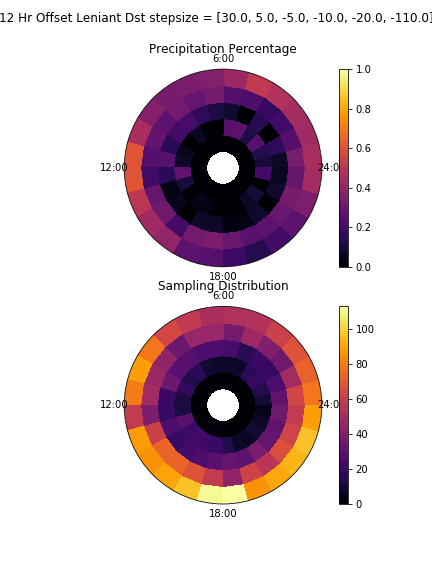
\includegraphics[width=\linewidth]{12DstOffsetStrict}
        \caption{Minimum Dst 12 hours prior}
        \label{fig:dst:c}
    \end{subfigure}
    \caption{Dst}
    \label{fig:dst}
\end{figure}



\begin{figure}[h] % ! overrides latex, h here, t top, b bottom, p special page for floating objects	
	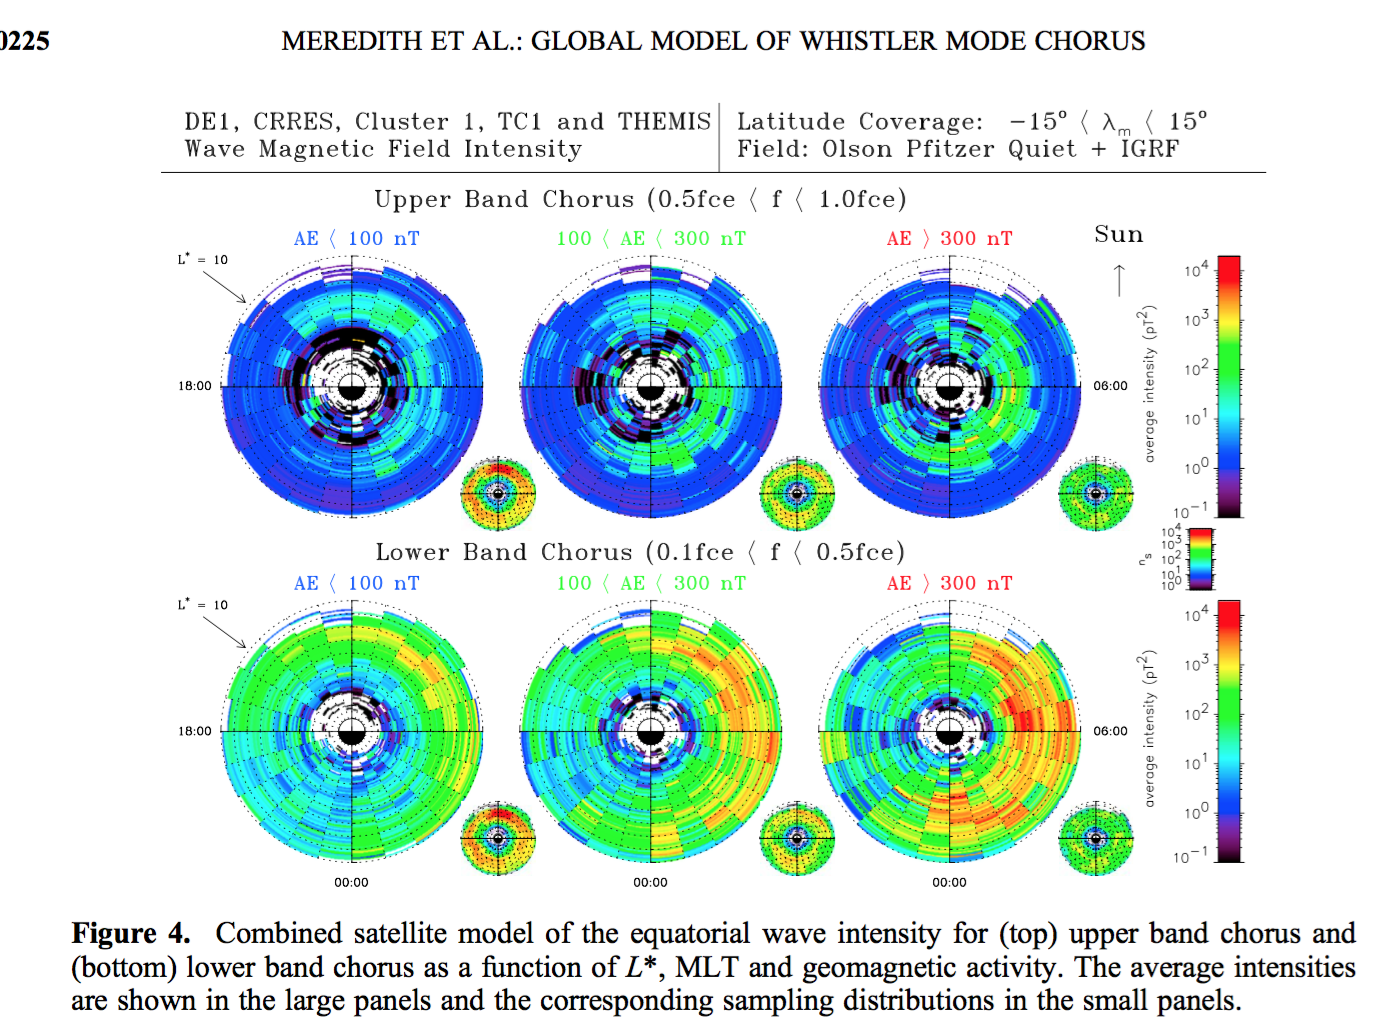
\includegraphics[width=\textwidth]{Meredith2012chorus} % adding right pushes my fig to the left wtf
	\caption[Short caption]{\textit{Global distribution of Upper/Lower Band Chorus [Meredith 2012]}}
	\label{fig:meredith}
\section{Discussion}
\mypara In the distribution of upper and lower band chorus in Figure \ref{meredith} from [Meredith:2012] it is suggestive to look at the global distribution of chorus waves and compare to our results. Now, if we look at the appropriate L bin for PFISR in the Meredith figure, we see good agreement between the distribution of upper and lower band chorus wave intensities and observed energetic particle precipitation for high AE and Dst values, so high geomagnetic activity. This was very interesting after looking at the Thorne 2010 paper where they showed that chorus waves were the dominant cause of the diffuse aurora, which is considering particles in the 0.1-30 keV energy range. But EPP in the D-region is considering looking at energies > 30 keV and the distribution of precipitation still seems to match the distribution of chorus waves, albeit for high geomagnetic activity. Thus Chorus waves are the dominant cause of EPP. 

BOOM *drops mic*... Oh wait, that's not how it works? Darn :/
\end{figure}


\end{document}